\section{Results}
\label{sec:results}

\subsection{Questionnaire respondents}

A total of 30 respondents submitted their responses to the online questionnaire. Five responses were discarded due to extreme values, inappropriate comments, or for falling outside of the target user group. The remaining 25 consisted of individuals holding professional roles in pathology or neuropathology, either as a consultant (12), researcher (6), pathologist in training (4) or laboratory technician (3). 

Of these 25 respondents, 12 considered themselves familiar with the application of AI in pathology, with 16 reporting having used AI solutions in routine diagnostics (6) and/or research (13). 13 respondents considered themselves familiar with ML, with a strong rank correlation between AI and ML familiarity (\(\rho = 0.6\)). AI familiarity data was missing for two respondents.

Most respondents reported using digital pathology and/or telepathology either in research (12), routine diagnostics (3), or both (6). Only four reported working solely with analogue methods, all of whom also reported not using AI methods at all in their work. 

\subsection{Interview participants}

Six certified pathologists (denoted P1--6) participated in face-to-face interviews, each lasting around 60 minutes. All interview participants were involved with research in pathology in some capacity, and three were currently involved in routine clinical practice. Years of experience as a certified consultant ranged from one to 45, with one participant being the current director of pathology, another a retired director, at major German research hospitals.

All participants of the interviews were familiar with the field of digital pathology and had some contact with AI applications, both in the research context (P1,2,5,6) and the applied and regulatory context (P3,5,6). Three participants reported being familiar with AI, but only having limited knowledge of the internal workings of it (P1,2,5). Furthermore, two participants (P5,6) reported having applied AI solutions to routine diagnostic tasks, albeit with unsatisfactory results. P3 and P4 had not seen or completed the questionnaire beforehand; all other participants had.

\subsection{Explanation classes}

\begin{figure*}
\centering
\begin{minipage}[c]{0.9\textwidth}
    Trust Scores:
    
    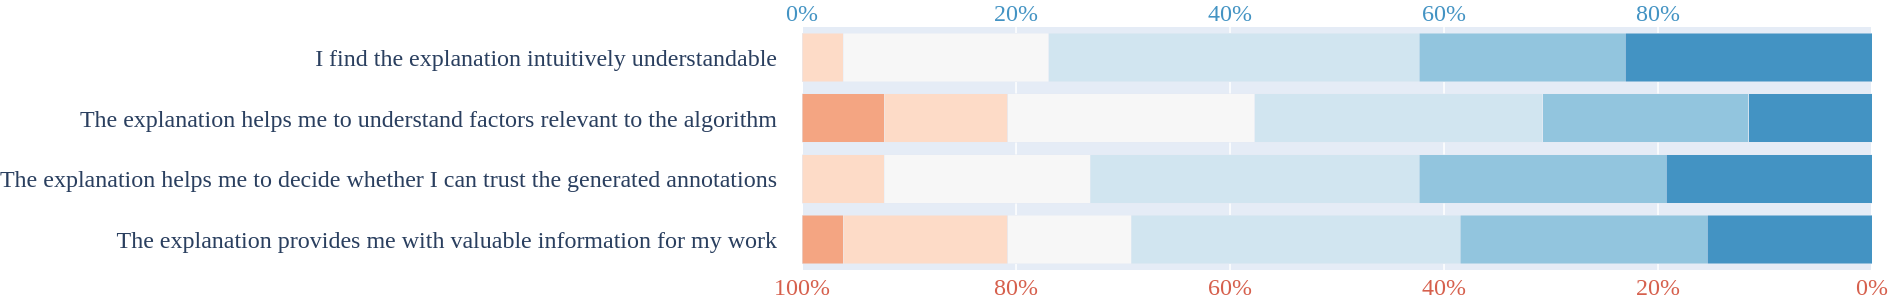
\includegraphics[width=\linewidth]{main/Graphics/4ResultsandAnalysis/0_TrustScores.png}
    
    Counterfactuals (One-axis):
    
    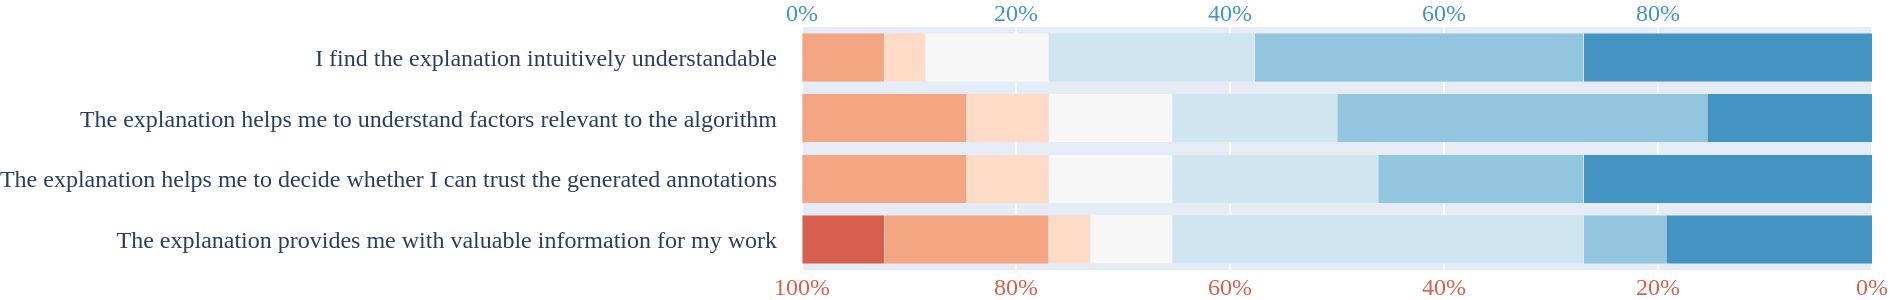
\includegraphics[width=\linewidth]{main/Graphics/4ResultsandAnalysis/1_CounterfactualsOneaxis.png}
    
    Concept Attribution:
    
    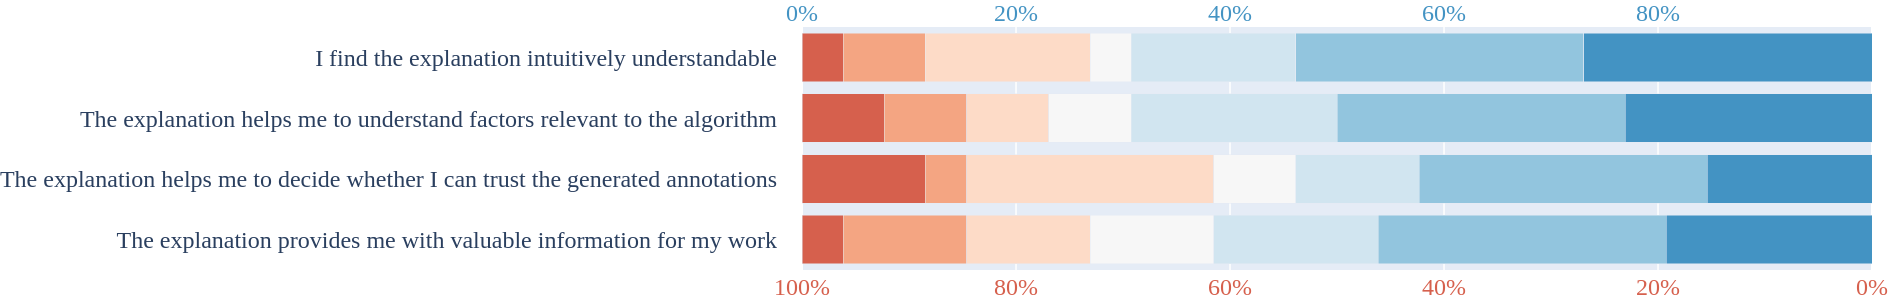
\includegraphics[width=\linewidth]{main/Graphics/4ResultsandAnalysis/2_ConceptAttribution.png}
    
    Counterfactuals (Two-axis):
    
    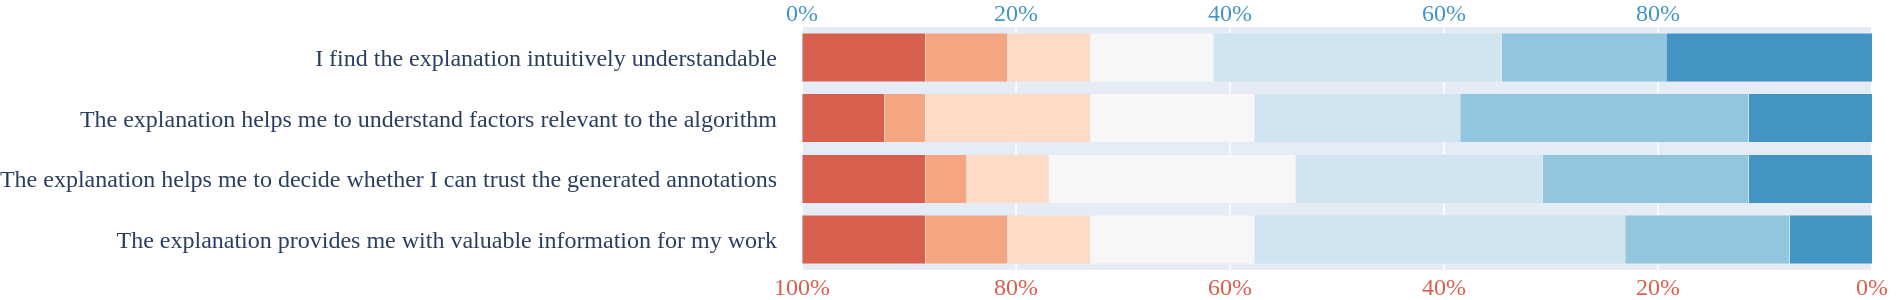
\includegraphics[width=\linewidth]{main/Graphics/4ResultsandAnalysis/3_CounterfactualsTwoaxis.png}
    
    Prototypes:
    
    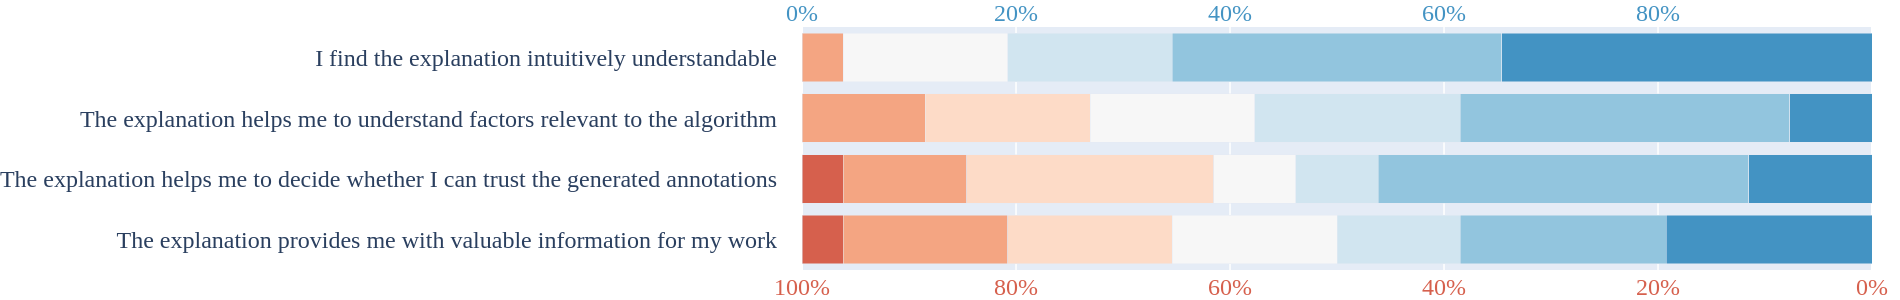
\includegraphics[width=\linewidth]{main/Graphics/4ResultsandAnalysis/4_Prototypes.png}
    
    Saliency map (Global):
    
    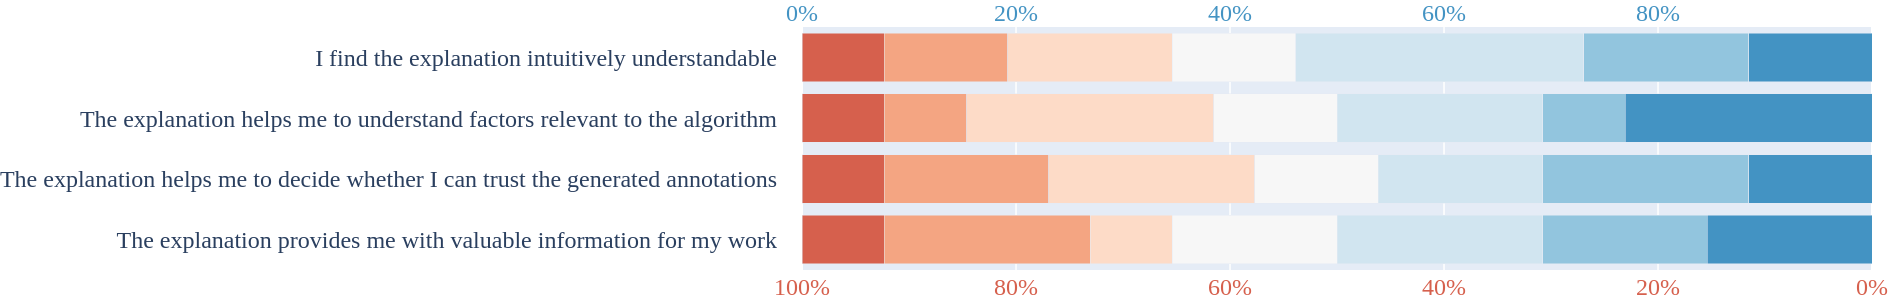
\includegraphics[width=\linewidth]{main/Graphics/4ResultsandAnalysis/5_SaliencyMapGlobal.png}
    
    Saliency map (Local):
    
    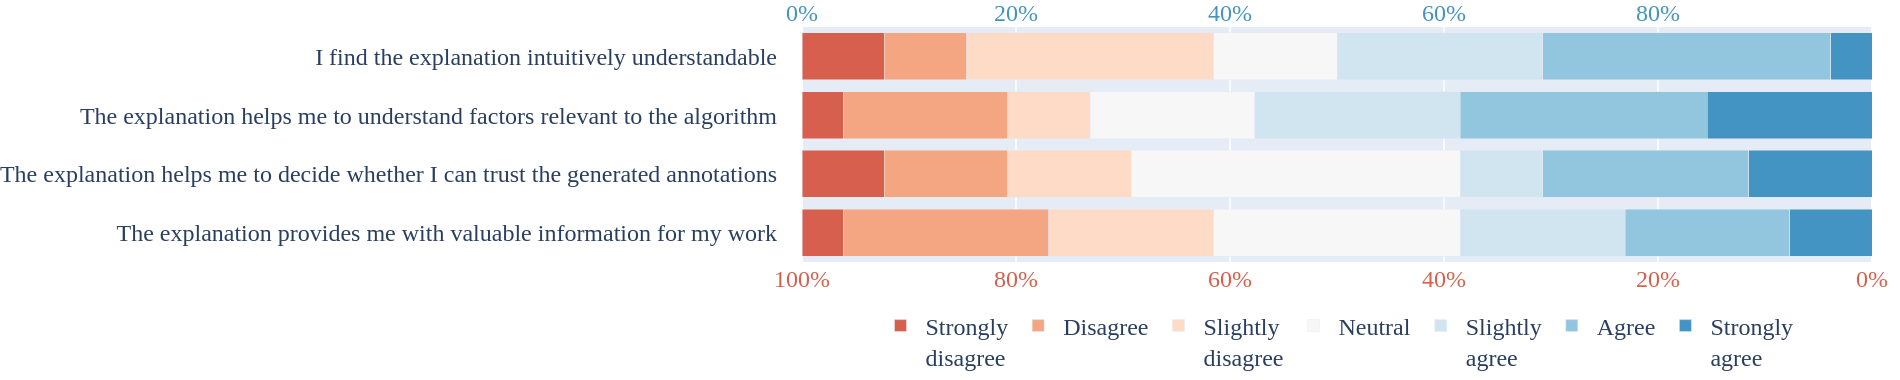
\includegraphics[width=\linewidth]{main/Graphics/4ResultsandAnalysis/6_SaliencyMapLocal.png}
\end{minipage}
\caption{Questionnaire results in descending order of agreement with the value question} %TODO wording
\label{fig:results}
\end{figure*}

\subsubsection{Trust scores}

% \begin{figure*}
%     \centering
%     \includegraphics[width=0.8\textwidth]{main/Graphics/4ResultsandAnalysis/TrustScoresBorderlineCases.png}
%     \caption{.}
%     \label{fig:trustscores}
% \end{figure*}

The indication of low- and high-confidence annotations was regarded as being intuitively understandable, a sentiment corroborated by 76\% of the survey respondents (see figure \ref{fig:results}), even as being described as ``almost too basic [to be considered an explanation]" (P5). 

% Understandable:
% + “This is nice and understandable” (color coded highlighting of annotations) P3 76% of survey
% + Almost too easy/basic, nice because it’s straightforward P5

Aside from identifying high and low confidence annotations, many participants also inferred from this the factors that may have been important to the solution, linking low-confidence annotations to the presence or absence of certain features (P1--3,6); ``[I] can see from this that the staining intensity was important, but the size was not'' (P6).

% Helps understand factors
% * Also informative about important factors behind model output, i.e. uncertain cases linked to e.g. nuclear irregularity. P1, 2 “I see what is the basis for decision” P3 
% * “Can see from this that the staining intensity was important, but the size was not” (small cells that are highly stained, were considered positive, “I would challenge that”) P6

All interview participants indicated that seeing the confidence of annotations (or at least, seeing which were low confidence) helped to deciding whether to trust the results. On the one hand, this stemmed from the implied ability to choose what to do with these low-confidence annotations; e.g. to accept, discard or manually change them (P1--5), or to further adjust parameters and thresholds (P6). On the other hand, the coincidence between annotations that were labelled low-confidence and those that the pathologist would also ``have difficulties with" (P1), this also increased their trust in the AI solution (P1,2,5,6). One participant explained this in terms of giving them the feeling that the AI solution was ``doing the same things that I do" (P2). 

% Helps me to decide whether to trust:
% +Good to understand decision boundary P1
% + This would give me confidence in using the result, or in deciding to not use it P6 72% of survey
% * Immediate comparison between ambiguous cases for model vs pathologist self, highlights importance and difficulty of staining intensity.“I can see where the limitations are and also where I would have difficulties in choosing” P1 ”is it similar to mine” “doing the same things that I do” P2, Take a glance and say ‘this fits with my interpretation’ P5

Overall, being able to see the low-confidence annotations was deemed valuable by all participants for the purposes of assessing the AI output, particularly in conjunction with other explanation methods (P4--6), or as a final check before deciding whether to accept the results (P6). Some went as far as to say ``the way it is presented, I would know at a glance whether I accept this evaluation" (P6); ``[I can] take a glance and say ‘this fits with my interpretation’" (P5).

% Is valuable
% + Very useful to know the limits, to know where to double-check, can decide whether to include low-confidence or not P1, 2, 3, 4, 5
% + “I would decide whether these weakly stained should be counted or [not]” P2,3
% +  Good add-on to prototype P4
% + For the end, it’s a very good idea (after manipulation of thresholds). Then make a diagnosis (also depending on task, sometimes anything above 1% is a positive, sometimes more nuanced). P6
% +The way it is presented, I would know at a glance whether I accept this evaluation (in this case I would question it) P6

In terms of criticism for the approach, it was suggested both in interviews (P2, 3), as well as in the questionnaire comments, that this implementation would need confidence indicators for the negative annotated nuclei in order to effectively assess the AI output. A proposed improvement would be to display low/high confidence annotations for both positive and negative annotations (P2,3); for instance, separately or using different color schemes. As well as having the option to manually resolve low confidence annotations, it was also presumed that manual reviewing these annotations would (or should) also help train the AI solution (P1, 6).

% Would be better if
% * Separate out into different classes +ve/-ve. P2, C, P3
% * Great to have the possibility to interact, resolve uncertain cases to help algorithm improve. P1,

Aside from per-annotation confidence scores, there were many comments pertaining to the kind of information about overall model confidence, validation, training data, etc. that was was identified as important for building trust. This topic is discussed in more detail in section \ref{sec:otherideas}.

% * More general, knowing how a model was trained is important, ground truth annotations: human, more than one, from same institute, or more than one? P1


\subsubsection{Concept attribution}

% \begin{figure*}
%     \centering
%     \includegraphics[width=0.8\textwidth]{Graphics/4ResultsandAnalysis/ConceptAttributionText.png}
%     \caption{caption here}
%     \label{fig:conceptattribution}
% \end{figure*}

This example was widely considered intuitively understandable, as well as informative about the factors important for the AI output, albeit not in a way that was particularly useful (P1,2,4--6). This sentiment was reinforced by the questionnaire results, where 68\% of respondents agreed that the explanation was intuitively understandable (statement 1), with a low rank correlation between this and its perceived value to the user (statement 4) (\(\rho_{1,4} = 0.38\)).

% This is understandable/  
% Understandable (but often not useful) P1, 2,4,5,6 + 71% of survey, but with a rank correlation of 0.3 to its value
% Helps understand factors:
% + Informs about factors that were important P2, 4, 5 71% of survey with a 0.53 rho vs value

In spite of this ambivalent reaction to the explanation, some respondents pointed out that it would still instill trust the AI output (P2,6); ``seeing the same factors that I find important makes me more confident in using the information that is provided, if I know that the application uses the same information that I would, as a human being. And applying the procedures that you are applying" (P6).

% Helps me to decide whether to trust:
% + Helps to build trust P2, 6
% + Seeing the same factors that I find important makes me more confident in using the information that is provided, if I know that the application uses the same information that I would, as a human being. And applying the procedures that you are applying. “Makes me feel that I’m looking at something that I, as a pathologist, would apply within seconds to this image.” P6

It was suggested that this explanation has some value as a sanity check, making clear whether an important factor is being `missed' by the AI solution (P1,4). However, in both cases it was also pointed out that such sanity checks should not be necessary with a well-validated, clinically approved solution.

The main criticisms for the explanation were the lack of precision and/or descriptiveness (P1--3), that having to read text is generally undesirable in the pathologist workflow (P3,4); ``a picture is worth more than a thousand words" P3; or that it is simply not well-suited to this particular task of Ki-67 quantification (P2, 4--6). 

Regarding the lack of precision, it was pointed out that the explanation does not tell you how these factors affect the results, where the thresholds are, whether it is increasing or decreasing them that has an effect (P1, 6). A comparison was drawn between how a pathologist would explain what was important to them using descriptive language, and that this falls short of that level of precision (P1).

On the other hand, it was suggested that the explanation method is fundamentally promising and could be valuable with refinements (P2--6). Suggested improvements included showing factors in combinations (P2) and/or with finer granularity (P6), or moreover, with indications of thresholds and visual examples demonstrating how these changing factors affect output (P2, 6), or in combination with an interactive tool for changing these thresholds (P6). % note this tending towards CF in discussion

It was suggested that this type of explanation may be more suitable for other diagnostic tasks; for example, in tasks involving differentiation between metastates and lymphocytes in lymph node sections, where other factors such as cell size, regularity are more important than in the Ki-67 quantification case (P2, 4--6).

% Is valuable?
% + Fine as a sanity check (but should be unnecessary) P1,4
% + The concept for [explaining] is good here P3, C 62 % of survey
% - for this particular problem, this does not give me information I need P1, 4
% - Don’t want to spend time reading “One image is more than a thousand words” P3, 5
% - there could be quite a lot of additional factors, or combinations of factors, so this would need some supervision C, P2
% - for this particular problem, this does not give me much information P1, 3
% - Don’t know what intensity is meant here, not precise enough P3
% Would be better if:
% * more descriptive, but maybe at the cost of intuitiveness? P1, 3
% * What is it about the straining intensity, eg? What is the threshold, what would have to change? % * Compare with talking to a pathologist. Pathologists used to being descriptive, always comparing, how detailed would a pathologist be? Becomes similar to a generated report, which is useful, insofar as a report is. how is it learning to make this description, outside scope of the task P1, 6
% * could be very valuable with finer granularity with quantitative information about the boundaries, maybe displayed with visual examples. The solution should be able to point out examples of different features (very round nucleus, very irregular, ones in-between) ie. tending toward counterfactuals P2, 6
% * could be useful for classification task, eg. tumor vs normal tissue, cell type. Not so useful for staining. In a more complex case, lymph node. High proportion of Ki-67 stained lymphocytes, alongside cancer cells/metastases. How to differentiate between stained lymphocytes and cancer cells is important, can’t just be on the basis of staining intensity, e.g. size of nuclei, comparison with staining in areas that are definitely non-tumour. P2, 4, 5, 6
% * if you are able to manipulate these factors, if you move these from left to right, how does the proportion of tumour cells eg. change P6

While narrative report generation through identification of text attributes was not deemed to be particularly useful (P1,5), the use of text-based explanations or descriptors to the generation of synoptic reports was mentioned (P3,5,6). This is discussed further in section \ref{sec:otherideas}. %TODO refer back to this

% Other comments:
% * Not necessary for synthetic reports yet, could be valuable for structured reporting, but we are the ‘very beginning’ P3
% * Taking up the role of cytoscreeners, giving morphology labels, justification for classifying regions as tumor/non-tumor P5

\subsubsection{Counterfactuals}

All interview participants indicated to some degree or another that the one-axis variant is immediately understandable; ``within a fraction of a second, I can see whether I agree with this or not" (P5); ``Immediately I know why half of the (negative) cells are missing" (P1); with many indicating that the two-axis explanation was not as clear as, or potentially more confusing than the simpler variant (P2--5). This was corroborated in the questionnaire results.

% Understandable
% + 75% of survey (58% for 2-axis)
% + Very straightforward, in a fraction of a second I can say whether I agree with this or not P5
% + “the difference between positive and negative is completely clear" P4
% - What is a counterfactual? Don’t understand this question (comments)
% - 2-axis case not as intuitively understandable, potentially confusing P2, 3, 4, 5 29% of survey
% - Not immediately clear that this is generated data P2
% - hard to distinguish between factors that are changing P2, 3

Interviewed pathologists were almost unanimous in their agreement that the explanation ``helps me understand what the algorithm is looking for” (P1), going so far as to claim that ``this is enough to understand [the result]" (P3). All participants drew some concrete conclusions about the factors important to the AI solution, finding it self-explanatory that staining was the most important factor distinguishing positive from negative marked nuclei, with some identifying other important factors such as shape, size of nuclei, particularly in separating the positively annotated from the unclassified nuclei (in the two-axis example) (P1--3).

% Helps understand factors
% + one-axis 62% agreement with rho 0.72 vs value
% + Immediately I know why it missing half of the (negative) cells are missing  (1 axis),  P1
% + ``this helps me understand what what what the algorithm is looking for”P1, ``This is enough [to understand the result]"P3 (1-axis) P1,3,4, 5
%  + Helps to understand that the staining intensity is important P2, nucleolus seems to disappear P2 ,“I think the algorithm is looking for shape and for darkness” (2-axis) P3,
% The most important thing between positive and unclassified is the shape  (2-axis) P3
% + understandable, what kinds of cell it is using to assign +ve/-ve label P2
% +  ``This helps me understand more the +ve labels” (2-axis) P1  
% * Perhaps cluster is too small to be tumour cells (2-axis) P2 

The ability to clearly see the boundary between positively and negatively annotated nuclei was widely considered as an important aid to trusting the AI output for the specific task of quantifying Ki-67 positivity of cancer cells. It was noted that there is another aspect to this task, in deciding which of the nuclei in the slide belong to tumor vs non-tumor cells. 

Some indicated that the two-axis variant helped them to trust that the solution was making this distinction based on the right factors (P3), or at least, was having the same difficulties in making this distinction that they would (P1,5). One participant also suggested that this is not an issue, as the recognition of tumor vs non-tumor cells is a separate upstream task that would have already been completed by this point “Once I’m at IHC, I’m just looking at positive or negative” (P5).

% Helps me to decide whether to trust:
% + one-axis 62 % agreement with rho 0.84 vs value
% + It helps me know whether I can trust that the threshold is in the right place (1-axis) P1,2, 4
% + Inflammatory cells can stain, explanation shows the model also counts stained inflamm. cells P1, tells me that positivity is influenced by inflammation, also something that we have difficulty with P1
% + ”This gives me more information" (2-axis) P1 
% + Knowing where the algorithm has difficulties, and especially, that it has difficulties with the same things, improves trust > as it informs where you should ‘double check’ P1, 5

There was a consensus amongst participants that these explanations, or at least the one-axis variant, were a valuable method for understanding and knowing whether to trust the AI output for this particular task. Referring to the two-axis variant, one participant stated “I think ... this one is the one that provides me all the information I need to make an assessment about the results that the algorithm is giving me, based on my own way of accessing [this task], and the pitfalls that I know are there ... because it's also all the information that I use on my own" (P1); another ``I know [artefacts] aren’t being included in the decision because they aren’t shown in the explanation" (P3). 

It was noted by many participants that the one-axis case could be more useful due to its simplicity (P2--5), a sentiment backed up by the questionnaire results, in which the two-axis variant rated significantly lower on Q1.

% Is valuable:
% + Very nice image (1-axis) P1, 5, 6
% +  “This one is the one that provides me all of the information that I need, based on my own way of accessing this and the pitfalls that I know are there”. “B/c it is all the information that I use on my own, and the pitfalls that I have and that the algorithm will also have” P1
% + initial reaction is that interpolation is useful C
% + subsumes prototype explanation P4
% +  Unclassified result is important, as it is important to have a check on what kinds of objects were not detected/classified. P4, 5
% - But I think 2-axis is too much information, simpler example is better P4, 5
% * re: 2-axis: ``This is an add-on [to the simple case]" (2-axis) P3

Aside from this, other pitfalls were noted by participants. It was not self-explanatory that the intermediate images were synthetic (P2), and that it was not clear which other factors apart from staining intensity were changing between the positive and negative cases in either variant (P2,3). It was also suggested that the explanation could be distracting, causing a pathologist to spend too long scrutinising the exact position of the decision boundary shown in the explanation, at the expense of looking at the slide itself (P4).

% - Could be confusing, cause too much time to be wasted scrutinising the boundary in the explanation P4
% * does not tell us about characteristics of tumor cells, but that is fine, as this would have been an upstream process, to look at slide with H&E. “Once I’m at IHC, I’m just looking at positive or negative” P5
% * doesn't give the full picture of possible negatives; many counterfactual examples that are more closely related to the positive example which could be useful for understanding the nuances and building trust (comments)

% * It would be lacking if there were not the two labels (+ve and -ve) [because -ve cells are important for ki-67) P1
% * [useful] at least in this area, might not apply to outside
% * Negative results could be due to disagreement with the actual result shown. Should be considered as a tool with which to interact with the AI, not as a ‘truth’ P6

It was suggested that the explanation could be improved by showing an ensemble of counterfactuals, to try and explore the different factors that are changing between positive and negative (P2, 6). Comments from the questionnaire reinforced this idea, suggesting that it would be valuable as an interactive tool with the ability to select different nuclei as a starting point for the interpolation to counterfactual classifications. It was also suggested that the on-slide control should also be displayed for comparison (P6).

Many participants mentioned the possibility of interactivity, with one taking it a step further, in suggesting that this explanation should only be used as a tool to interactively refine the decision boundaries, not as a source of explanation in itself (P6). Along these lines, they also suggested that this would be a valuable tool for refining multi-modal decision boundaries, e.g. in HER2 grading where, unlike Ki-67, the intensity of staining holds clinical relevance.

% Would be better if:
% * An ensemble of many counterfactual examples/factors of variation P2,
% * Interactive, presenting additional examples and asking for interaction from user, do you [user] agree with the intermediate results? For every slide when an analysis is done on a whole slide, to do an internal quality assurance. Does the pathologist agree/not agree, before releasing result, and to improve the algorithm for the future P2, 6 (especially 6)
% * Comparison with on-slide control

% Would also be useful in this context:
% * therapeutic antibodies (eg HER2) with multiple grades 0, 1+, 2+, 3+. Helpful to adjust the AI application. P6

\subsubsection{Prototypes}

% \begin{figure*}
%     \centering
%     \includegraphics[width=0.8\textwidth]{main/Graphics/4ResultsandAnalysis/PrototypesHighestconfidence.png}
%     \caption{.}
%     \label{fig:prototypes}
% \end{figure*}

The majority of participants in both the interviews and online questionnaire found this explanation intuitively understandable (P1,2,3,6), with 80\% of the latter agreeing with the first statement to this effect. However, this ease of intelligibility correlated poorly with its perception as being a valuable explanation (\(\rho_{1,4} = 0.31\)). The explanation was described as “precise, short and understandable, and reflecting the thinking of pathologists” (P3); “Simply understandable for a human being” (P6).

% Understandable
% + Intuitively understandable, agree with positive and negative prototypes P1, 2, 3, 6 + 80% of survey, but with a 0.31 rank correlation with it value, and a low correlation with any other attributes (factors, trust)
% + Correspondence with prototypical mental model of cell type (with proviso that people function in different ways). P1, 2, 3
% + “Precise, short and understandable, and reflecting the thinking of pathologists” P4 “Simply understandable for a human being” P6

Aside from helping the user to understand the ``perfect positive and negative result" (P1); ``heaven and hell" (P6), many participant also drew conclusions from this explanation about the specific factors that were important to the AI solution. For instance, that the prototypes shown underlined the importance of staining intensity over other factor (P2,6), ``size, shape, structure and color -- these are also the features you would focus on as a pathologist” (P3), or even indicated where threshold between positive and negative annotations lay (P5,6). It was pointed out that the explanation did not explain why cells were detected as tumor cells (P4).

% Helps to understand factors
% + Understand the ‘perfect’ +ve and -ve result, “Heaven and hell” P1, 6
% + Underlines the importance of staining intensity, rather than other features P2, 6
% + “I see that the algorithm has really concentrated on the point, what is [prototypical]” P3
% * Size, shape, structure and color “these are also the features you would focus on as a pathologist” P3
% - Does not explain why many cells are unclassified P4

All participants expressed at some point that seeing prototypical examples can help to inform a user's trust in the AI output, with some explaining this with respect to whether they reinforced the idea that the solution was taking into account the same factors as a pathologist (P1,3,4,6); “you feel better if you understand that the computer is evaluating something that you also do evaluate” (P6); ``If the [prototype] is not fitting to my understanding [of what it should look like], I know that the result can't be right" (P4). 

% Helps me to decide whether to trust:
% * Helps build trust in model output (later retracted) P2, 5
% * Helps build trust in model output P3
% * Reinforces the idea that the algorithm is taking into account the same factors as a pathologist P1, 3, 6
% * “you feel better if you understand that computer evaluates something that you also do evaluate.” P6
% +  If the positive and negative prototypes differ from the prototypical examples that I expect, it can tell me that there is a problem P4
% + ``If the [prototype] is not fitting to my understanding [of what it should look like], I know that the result can't be right." P4

Despite this, there was little consensus that this type of explanation was valuable, with the common criticism that prototypical results do not reflect the diversity that is central to pathology (P1,5,6) and/or that the information communicated is too trivial to be useful (P5). Some participants who identified the explanation as having some value in informing trust in the AI solution, later retracted this statement after identifying that the prototypes do not give indicate where the boundary between classifications lies, despite their expectations to the contrary (P2,5); ``If you show me the prototypical positive result, I would expect anything less to be negative" (P5). The risk of positive confirmation bias was pointed out by several participants (P1,2,5), leading one participant to name this as ``maybe the worst [explanation]" due to its potential to mislead (P5).

% Is valuable:
% - Hard to imagine useful contexts, pathology is about diversity. P1, 5, 6
% - nothing is black and white, prototypical example do not reflect the true result P1, 5
% - Strong risk of confirmation bias P1, 2, 5 , 6
% - Could be applicable where only the most strong staining (eg.) should be regarded as positive. If you show me the prototypical positive result, I would expect anything less to be negative — meta: after discussion realised that this did not show this, therefore misleading (“maybe the worst” explanation!) P5
% - I don’t get any useful information, anyone can say what the prototypical positive result is, more important to see the intermediate cases P5

On the other hand, one participant suggested that having the prototypical results was valuable as an indicator of the slide quality, more than the quality of the AI output; i.e. if they prototypical examples do not match the pathologist's expectations, it can indicate that there is an issue with the slide preparation and staining (P4).

% + Explanation as a means to check whether the staining is ok, slide preparation steps, not just to inspect AI P4

Several participants suggesting, either implicitly or explicitly, that a counterfactual-based explanations would be a more useful extension of this type of explanation (P1--3,5,6), either citing the examples presented, or describing their own variation on this theme. One participant suggested that it was useful to have both types of explanation together, with the implied option of being able to switch between them (P3).

% Would be better if:
% + Prototypes showing how it’s identifying cancer cells, counterfactuals showing it is making the distinction between negative and positive P3
% * It were the cf example P1

It was suggested that this type of explanation may be more suitable for tasks involving automatic detection of several similarly-presenting cell types, distinguishable only at high magnification (e.g. lymphocytes and plasmocytes). In this case, having the prototypical examples of each cell type could give the user confidence that the AI solution was correctly resolving the different cell types, without the need for laborious manual inspection (P1).

% * Useful in context: seeing prototypical results demonstrating key features (presence of nucleolus, cytoplasm), between very similar results > ie. prototypes of edge cases, boundary cases (tending toward CFs) Example: diff. Lymphocytes from plasmocytes, subtle difference, hard to distinguish at low power, even at high power non-trivial. Having prototypes helps lend confidence that the LC and PC (‘football’ pattern staining in latter) are being resolved from one another. P1


% * An ensemble of prototypical examples shown > selecting the ones you don’t agree with. e.g. as internal quality control P2, 4, You would need an array of ‘prototypes’… varying according to many different factors, then manipulating the limit, getting feedback on nuclear positivity as a function of this limit (with counterfactuals as an interface) P6

\subsubsection{Saliency maps}

% \begin{figure*}
%     \centering
%     \includegraphics[width=0.8\textwidth]{main/Graphics/4ResultsandAnalysis/SaliencyMapsGlobal.png}
%     \caption{.}
%     \label{fig:saliencyglobal}
% \end{figure*}

% \begin{figure*}
%     \centering
%     \includegraphics[width=0.8\textwidth]{main/Graphics/4ResultsandAnalysis/SaliencyMapsLocal.png}
%     \caption{.}
%     \label{fig:saliencylocal}
% \end{figure*}

The reaction of interview participants to these two explanation examples ranged from explicitly stated as being difficult to understand, distracting or confusing (P1,2,5) to being trivial to understand but not at all useful (P6). Some participants found the explanation interesting, but did not know exactly what to interpret from it (P4,5). One participant pointed out that it was not clear what was meant by 'the most relevant pixels' (P6).

% Understandable
% - Not easy to understand, distracting, confusing P2, 5
% ``I really don't know how to interpret this" P5
% - What do you mean by most relevant pixels…. ? P6
% * trivially understandable, in that it shows that this is a nuclear stain, but that is not useful to me at all P6

Many participants identified factors that were important to the AI solution based on the pixels highlighted as most relevant, including presence, staining, size, and position of nucleolus, or the staining pattern within the nucleus (P2,3,5,6). It was also pointed out that the explanation was ambiguous: it was not possible to infer which of these different factors were actually important or implied by the explanation (P2,5,6).

% Helps to understand factors
% - Strongly marked nucleolus, Telling me that the nucleolus is important (maybe that this is why it missed some cells). wonder what it was about that region that was used? The structure, or the dark staining of the nucleolus, the color, size, position? Saliency map is ambiguous between all of these different features P2, 5, 6
% - I see [the] combinations of features in this special image [used] for making decisions P3, 5
% - Cf. ESDIP town square: nephrology: could not tell any different between the segmentation output and the explanation P2
% - Tells me that its a nuclear stain (ie not anything useful) P6

While most participants did not see this explanation as helpful in establishing the trustworthiness of the AI output (P1,2,4--6), some indicated that the congruence between their understanding of what parts of the image are important and those highlighted by the saliency map would help them decide whether to trust the output (P3). On the other hand, it was pointed out to be contradictory when saliency map and annotations did not align (P4), and redundant when they did; “what is output and what is explanation” (P1).

% Helps me to decide whether to trust:
% - Does not help me to trust this result P2
% -  I can see if these decisions were made on the right objects (likely misplaced?) P3
% + If the majority of the salient objects are not satisfying, I am not trusting P3

Accordingly, the majority of participants did not find this type of explanation valuable to them at all for this task (P1,2,4--6). Even for those who considered it to have some value in explaining the factors important to the AI solution, the modality was too detailed and/or too time-consuming (P4--6). Some thought that it might be useful in research (P4) or as part of a suite of tools (P3).

% Is valuable:
% - Not telling me anything useful for this task P1, 4, 5, 6
% - “what is output and what is explanation” P1
% - High risk of positive confirmation bias P1
% - Per-cell saliency is probably too much detail. (Local) C
% + Valuable tool as part of a suite P3
% + interesting P4
% - but doesn't help me in any way (in routine) P4, 5, 6
% - Too much information / too high cognitive load P4
% - By this point I’ve already made a decision, redundant P6

It was suggested that this form of explanation may be more suitable for classification tasks, where spatial features are more important than for the Ki-67 quantification case (P1,2,4,5). For instance, in the case where the output of an AI solution is the classification of a tumor over a large region. It was suggested that, a pathologist could be more likely to trust a solution if the salient regions indicated match their expectations (P1,3).

% Would be better if:
% * Could be useful for a classification task, rather than segmentation. ie. what type of tumor is this? “which cells is he (AI) using to make this assumption (classification)” More trustworthy if taking into account more of the tumor? < belies a potential for mismatch between how does pathologist understanding of ‘what the most important parts are’ correspond to the models’ understanding P1 (add more discussion from P1), 2,  where spatial features are important, or where and how much staining occurs e.g. in cytoplasm, not just whether. 4
% * Maybe interesting in research (with the idea that it gives an idea of ‘how positive’ the staining was to be marked positive) P4

The risk for positive confirmation bias with such explanations was also pointed out. ``[It] is hiding a lot of information. But it's, it's very tempting, because it's very simple" (P1), particularly for pathologists who are not familiar with techniques with which can be generated, or at least aware that there are many different ways to do so (P1). As such, it was suggested that this type of explanation should only be used as one element within an array of explanations, or as a final check (P1,3).

\subsection{General observations}

\subsubsection{Expectations of explanations}

Participants unanimously expressed a preference for simple, visual explanations; "Pathologists are always looking for visual things, matches thinking. Anything outside this modality is foreign." (P1).  Interactivity was an often cited as a desirable (P1,3,4), if not necessary (P6) feature; e.g. the ability to adjust the threshold and see the resulting output.

All participants at some point expressed that explanations tended to increase trust in the AI solution when they demonstrated it making decisions in a relatable manner; i.e. when it "it matches the way we are thinking when we see the image" (P1).

``I think you will always come down to what I'm used to do what I'm looking for. And that I will ... mirror this into the algorithm ... it's like when we are training a resident or showing a case to a colleague, you are also doing this to see if you can trust the other person. Do they evaluate things that you do? Are they looking for other things that you are not, so that you can learn from this one? So I think this is a little bit how we will interact with the algorithm. We are testing it like we would another pathologist." (P1)

% Trust coming when the AI solution seems to be 'thinking' the same way as the pathologist:
    % Trust AI solutions when they (seem to) match the thinking of the pathologist P1
    %  If it has the same trouble differentiating [as I do], then it’s probably doing the task right" P1
    % ``I think you will always come down to what I'm used to do what I'm looking for. And that I will ... mirror this into the algorithm to it's like, I'm, it's like when we are training a resident or or, or showing a case to a colleague, you are also doing this to see if you can trust the other person? Does they evaluate things that you do? Are they looking for other things that you are not so that you can learn from this one? So I think this is a little bit how we will also interact with the algorithm. We are we are testing it like we would another pathology." P1
    % Pathologists are always looking for visual things, matches thinking. Anything outside this modality is foreign. P1,3,5
    % * Computer scientists and pathologists looking for different things P1


% \subsubsection{Ability of pathologists to explain their decision}
% % Can't always just explain your decisions as a pathologist, a lot of intuition. But you always try, you can always pass some information onto pathologists, or there would not be any pathologists. P1
% % ``I think any experienced, experienced pathologist is able to explain his decision to another pathologist in a satisfying way that the other one will then agree or disagree with with, with this decision." P1
% % * Challenging to use language in explanations, in describing cases, before there is a standardised vocabulary (see structured reporting, DICOM 222) P3
% % * Not only a problem of explanations, but also a problem of observation P3
% % To explain decisions: highlight regions and making (simple) text annotation, with inset (P3,6)
% % To present a case, adding paired elements, you can describe a case completely. Also adding information about genomics, IHomics. P6

% % Since xAI solutions should use similar approaches to the modalities used by Pathologists to explain themselves (see Trust in AI, XY), an important point of inquiry was the way Pathologists would explain their own reasoning.

% Participants expressed that they were confident justifying their reasoning, but also noted that experience and gut feeling play a role at many decisions (P1, P3). The difficulty of non-standardized vocabulary adds to this problem of non-specificity (P3).

% For visual explanations, Pathologists declared that they simply highlight regions on WSI, preferrably with insets, and make simple text annotations (P3, P6). Furthermore, paired reports (as used in synoptic reports) can be used to describe cases (P6).

% \subsubsection{New approaches and how AI should be used}
% % -show real prototypes (Ri)
% % -AI as flag/second pair of eyes (P3) this is the idea behind synoptic reporting grid overlay P6 (referred to TNM staging.)
% % -

\subsubsection{Use of AI in pathology}
It was observed that the term 'AI' is vague,  particularly in light of the new definition of EU terminology \cite{ISO_IEC_22989}; ``Nobody knows what is artificial intelligence. Nobody knows what is intelligence" (P3). It was noted that, according to this definition, AI has been applied to pathology for decades in the form of numerical modelling, regression, etc. Similarly, computer-assisted diagnosis has existed in some form or another for many decades, with image processing methods, counters, microscope-mounted cameras, etc., and the modern trend of deep learning applications to digitised slides is the logical next step in an ongoing process of innovation (P1,3).

% AI as extension of manual tools, counters, camera on microscope etc. - P1
% * EU publication of AI , much broader than ML - P3
% * Under new EU term definition, this has been going for the last 40 years - P3

AI solutions were often regarded as an extension of these manual tools, assisting with simple but time-consuming tasks (P1,3,6); e.g. counting cells or estimating percentages, etc. Speed was named several times as the highest priority for AI solutions, with the rationale that if the AI did not save the pathologist time, they would simply perform the task themselves (P4--6). The slide digitisation process itself was also named as a limiting factor; i.e. by the time a slide had been scanned and was ready to be viewed digitally and/or processed by an AI solution, the pathologist could have already completed the task under a microscope (P4). It was suggested that slide digitisation needs to reach a critical level of adoption ``over 90\%" in order for such applications to make sense (P6).

% It has to always save time. If it takes more time, I would just do it myself on my microscope P4-6 Or even that this is the only benefit of AI solutions P6
% * speed of pathologist diagnostic process was many times stressed, pointing out that AI solutions have to be incredibly fast in order to provide a benefit. P6
% Currently, using AI solutions takes much longer than manual handling, as digitisation process is slow P4
% Acceptance of digital pathology - benefit will be there if you avoid stacks of slides, but this requires >90% digital. The hospital pathologist would still rather work with a microscope, so it needs to reach a critical point of adoption. P6

One participant made the point that the pathologist's liability for their decisions, and therefore obligation to anyway check every result and slide, was a limiting the usefulness of AI solutions (P4,6). It was suggested that AI solutions could be useful as a backup, giving a second opinion or flagging features worth reviewing, even after the pathologist has made their own diagnosis. To this effect, the impartiality of AI solutions (for instance, to the seniority of the pathologist) was cited as a strength (P4).

% AI as an extra set of eyes. Maybe not so important for the clearly positive or negative cases, but valuable for flagging up where there is something that might have been missed, contentious cases P4
% Impartiality of AI solutions is a strength, does not care about seniority/experience of pathologist P4

Regarding the current state of AI solutions for pathology, limitations with regards to accuracy (P5) or data protection (P6) were cited as prohibitive for the use of commercial solutions in clinical settings. It was observed that it is not sufficient to ``buy [AI solutions] at the App Store" (P3), but rather that the techniques of machine learning must become part of pathologist's training in order for AI be effectively applied to pathology, and that the lack of mutual understanding between computer scientist and pathologists was a factor limiting adoption (P3,5).

% No suitable/usable solutions available currently P5
% * Pathologists must be trained in machine learning, AI should be included in the training programs of pathologists “You can’t just buy it at the App Store” P3
% Lack of understanding between computer scientists and pathologists P5
% Mesothelioma detection solution, good prognosis prediction, but not clear what features are being used. “Not sure who is learning here, we or machine” P5
% Many AI solutions cloud-based, due to continuous improvement, a problem for German hospitals due to breach of data privacy. Need to run solutions on local network. P6

% TODO: work on P4 00:45 onwards

\subsubsection{Use of AI in Ki-67 quantification}

The issue of inter-pathologist variability in Ki-67 positivity quantification was identified; ``[It] is very boring to count nuclei positive or negative nuclei. And most of these things are now based on on an estimations only, and therefore the results are very weak .... in breast pathology, there's a threshold of ki 67 positivity of 14.4\%, for selecting some kinds of patients to get chemotherapy or not, and nobody can [estimate] 14.4\% ... It is quite nonsense, but it is the official recommendation of some bodies in European and national pathology" (P1)

Some participants considered AI assistance to be a useful tool in mitigating this issue (P1--3), citing the ability of AI solutions to work systematically without becoming fatigued (P1,3) and the potential for them to make better estimations by taking into account other data modalities; e.g. cell morphology, molecular data (P2). 

% * “Ki-67 is a really bad example for AI” P3
% * Awareness of the limitations of computer-unassisted tasks P1

On the other hand, it was suggested that this task was too trivial for AI assistance to be useful (P6), or that lack of standardised training data represents a prohibitive limitations to their potential accuracy (P3). Another identified that the pathologist's fine-tuning of AI parameters (e.g. positivity threshold) would anyway reintroduce the same subjective variability, should they have this option (P2).

\subsubsection{Trust in AI solutions}

The pathologist's own judgement was cited as the primary basis for judging the accuracy, and therefore trustworthiness, of an AI system (P5,6). It was suggested that pathologists' trust in an AI solution would be established after extensive use, testing, and comparison with the work of multiple colleagues (P5).

External validation was commonly identified as a critical prerequisite to trust in an AI solution (1,2,4,5). It was suggested that AI solutions can and should be subject to more forms of validation than the work of pathologists normally would (P2). Diversity (P1,5) and experience (P6) of annotating pathologists were stressed as critical factors in assessing quality of validation and/or training data. Annotations from three pathologists, preferably all from different institutes, was suggested as a minimum requirement for trustworthy ground truth data (P1,5).

% Trust coming with experience, and historical accuracy, validation.
    
    % Trust comes with extensive testing, spotting issues, e.g. macrophage identified as tumor cell, tumor cell identified where there aren’t any, 1 tumor cell identified where there are 2 close together, etc… and comparing machine output with routine work of multiple pathologists — once I am comfortable, and if the software is fixed (not open for learning) then I can use these explanations to be happy at a glance P5
    
    % * Trust machines when they perform better, empirical basis, validation. P1,5
    % Would need to have all the information used by a solution to come to a conclusion PLUS validation. It’s not enough to just have one pathologist, one pathologist can be wrong. Need at least 3 pathologists, and compare the middle(e.g.) value with the solution. And who was the person (or people) who provided the input data. Size of cohort. A big different between molecular data coming from trusted institute, third party, commercial sources, etc. Some accessible explanations for how the solution works. All e.g.. in the form of a small brochure. And I would still validate it in-house, with these explanations as internal checks! (also backed up by early brainstorming session) P5 
    % Experience of training-data annotating pathologists P6
    
    % * Without even seeing the output, I would trust the results of a model using various annotation sources as [training] input rather than just one. Would like to see that more than one pathologist, from as many different institutions as possible. Consistency within institutions. P1

Participants expressed a range of attitudes toward relinquishing control of the decision-making process to an AI solution. Most participants expressed openness to an AI solution giving a contradicting result to their own (P1--5), with some identifying benefits in giving an AI solution more control over the decision-making process (P1--4), provided it was shown to be reliable. 

On the other hand, one participant expressed the expectation of always having the control over the decision boundary of an AI solution, although suggested that the parameters set by an experienced pathologist might then be used with confidence by one with less experience (P6).

The pathologist's legal accountability for their decisions was several times explicitly mentioned (P4,6), and used as a rationale both for (P4) and against (P6) endowing more control to an AI solution. 

% wrt. putting the AI in control:
    % * What would it take for you to put the machine in control?: additional methods of validations, aside from Ki-67 .. other antibodies, molecular methods addressing the same question — although these are not methods that a pathologist would use routinely to validate. P2
    % * ``No problem" to trust an AI to e.g. choose the threshold for Ki-67 positivity. I am just liable for the outcome. Just as much of a risk to change the threshold manually, as to trust the AI to do it. A good AI should choose the threshold - P4
    % The pathologist will always have to sign off on the result, even a bad result from an AI solution P6
    % I would never trust the threshold, I would always want to be able to manipulate it P6
    % As long as you are knowledgable as a pathologist, you need to anyway look and make a decision and check the result. “If you are relying on an AI solution to make a diagnosis that you cannot, you should give up on diagnosis and ask someone more qualified” P6
    % High importance of experience level of the pathologists who trained the solutions P6
    % * Human in the loop: if you can adjust threshold yourself, you are back to the same problem of variability/subjectiveness. Necessary for now, but eventually we should be tending towards ‘letting the machine’ choose the threshold, but right now too many confounding factors P2
    % Pathologist would tweak these parameters, threshold for various factors, to train the model. The most experienced pathologists would train the model, in order that less experienced pathologists can benefit from it P6
    % in the context of low/high confidence annotations: What would you do with low confidence nuclei? no good solution for deciding what to with results in ‘gray zone’, no consistent strategy. From AI solution, would throw out results. Link to variability between pathologists P
    
\subsubsection{Other suggestions for the use of AI in pathology}
\label{sec:otherideas}

Over the course of the interviews, participants suggested several potential approaches to explain or supplement AI solutions for pathology.

Several participants described variations on the theme of structured annotations (in the style of synoptic reporting) for the slides in question, providing additional context with which to evaluate and confirm the AI output (P2,5,6). For instance, allow a pathologist to quickly compare descriptors for regions marked by an AI solution as healthy vs. unhealthy (P6). It was implied that these annotations could be automatically generated, either based upon a body of machine-readable ground truth data (P6) or by combining the results of many other feature detection algorithms (P2). 

% combining synoptic reporting, clinical information, quality information, to add information to the image from the databank (e.g. quality information, “don’t look at this slide”, defect detection). Requiring cooperation between pathologists and IT experts. Building up a body of machine-readable data. Automatic annotations over slide. (P2, 5, 6) Accumulate observations in standardised language and look at frequency across the whole image P3
% Cross-referencing with other tissue features, an assay of KI approaches, taking into account other IHC stains, or from morphology in H&E. Detection of mutually exclusive features, detecting collisions. (P2)

Automated anomaly detection was also mentioned, wherein an AI solution might -- either as, or supplementary to, some other diagnostic output -- flag up features that are statistically rare and/or out of distribution for their training data, for manual review (P4,5).

% Anomaly detection with AI solution, pointing out out of distribution features, (P4) Detect everything that is not a “normal” cell and flag this up for inspection by a pathologist (P5)

A novel approach to explainability was suggested, wherein an AI solution could `explain' its decision by showing the images from training data that were most important for a given outcome, comparing this process to that of a pathologist referring to previous cases and reference material to justify their decisions (P1).

% Machine equivalent to showing reference examples, showing images from training data that most strongly informed a result, relatability to process a pathologist would go through (P1)

% TODO write about brochure
% now, how would it be format is not that doesn't help me because then I lost him. But if I'm if we're talking now really a couple of years ahead of us, and then you have really product which is ready to be whatever sold or marketing or put into marketing, then I would really like to have a small brochure I rarely write down. Okay, this was tested on so many 1000 samples with input from expert people that does not, they don't have to be topology. So pathologists, biologists and everything from this institution. And then our software was trained on this, we have been able to show this on this huge cohort, because for sauce writing cohort of 1000 is nothing. So and you cannot learn much after this. And that's why, and then you have we have Discord. And then it was validated in another independent group. And the results were very much similar concordant or something. So I would really like to have it as an end user to be really sure, but even with that, I was still validated in house. So I this is the, this is the same procedure with everything we buy very simple, this like antibody, which is ready to use or something, we still have to validate it to see if it's doing what they are selling it for. And we have to use our old cases where we are certain that it should be negative positive or something and that used, that's all.